\chapter{Theoretical Model}
The mathematical basis for \textit{Omnisoot} is explained in the top-to-bottom hierarchical order. First, the governing equations for constant volume, constant pressure, perfectly stirred and plug flow reactor models are reviewed in Sections~\ref{sec:cvr}-\ref{sec:pfr}. These equations differ from pure gas-phase transport formulation as they consider the solid phase. The transport equations of ``soot variables" include the source terms that account for change in each soot variable due to inception, surface growth, oxidation and coagulation. Then, particle dynamics models are explained in Sections~\ref{sec:particledynamics} that entails description of size distribution and morphology of soot particles and their collision rate, which is used to determine the coagulation source term. Section~\ref{sec:pahgrowmodel} focuses on the \textit{``PAH growth model"}s that take care of inception and adsorption from designated precursors and calculates the corresponding source terms. Similarly, the \textit{"surface reactions"} model are detailed in Section~\ref{sec:surfreacmodel} that elaborates on the surface growth and oxidation rates based on HACA mechanism. %Finally, the rate of addition or removal of gaseous species due to soot formation is explained in Section~\ref{sec:gasscrub}. 
Figure~\ref{fig:structure} illustrates the general structure of Omnisoot and the sub-models.

\begin{figure}[!htbp]
	\centering
	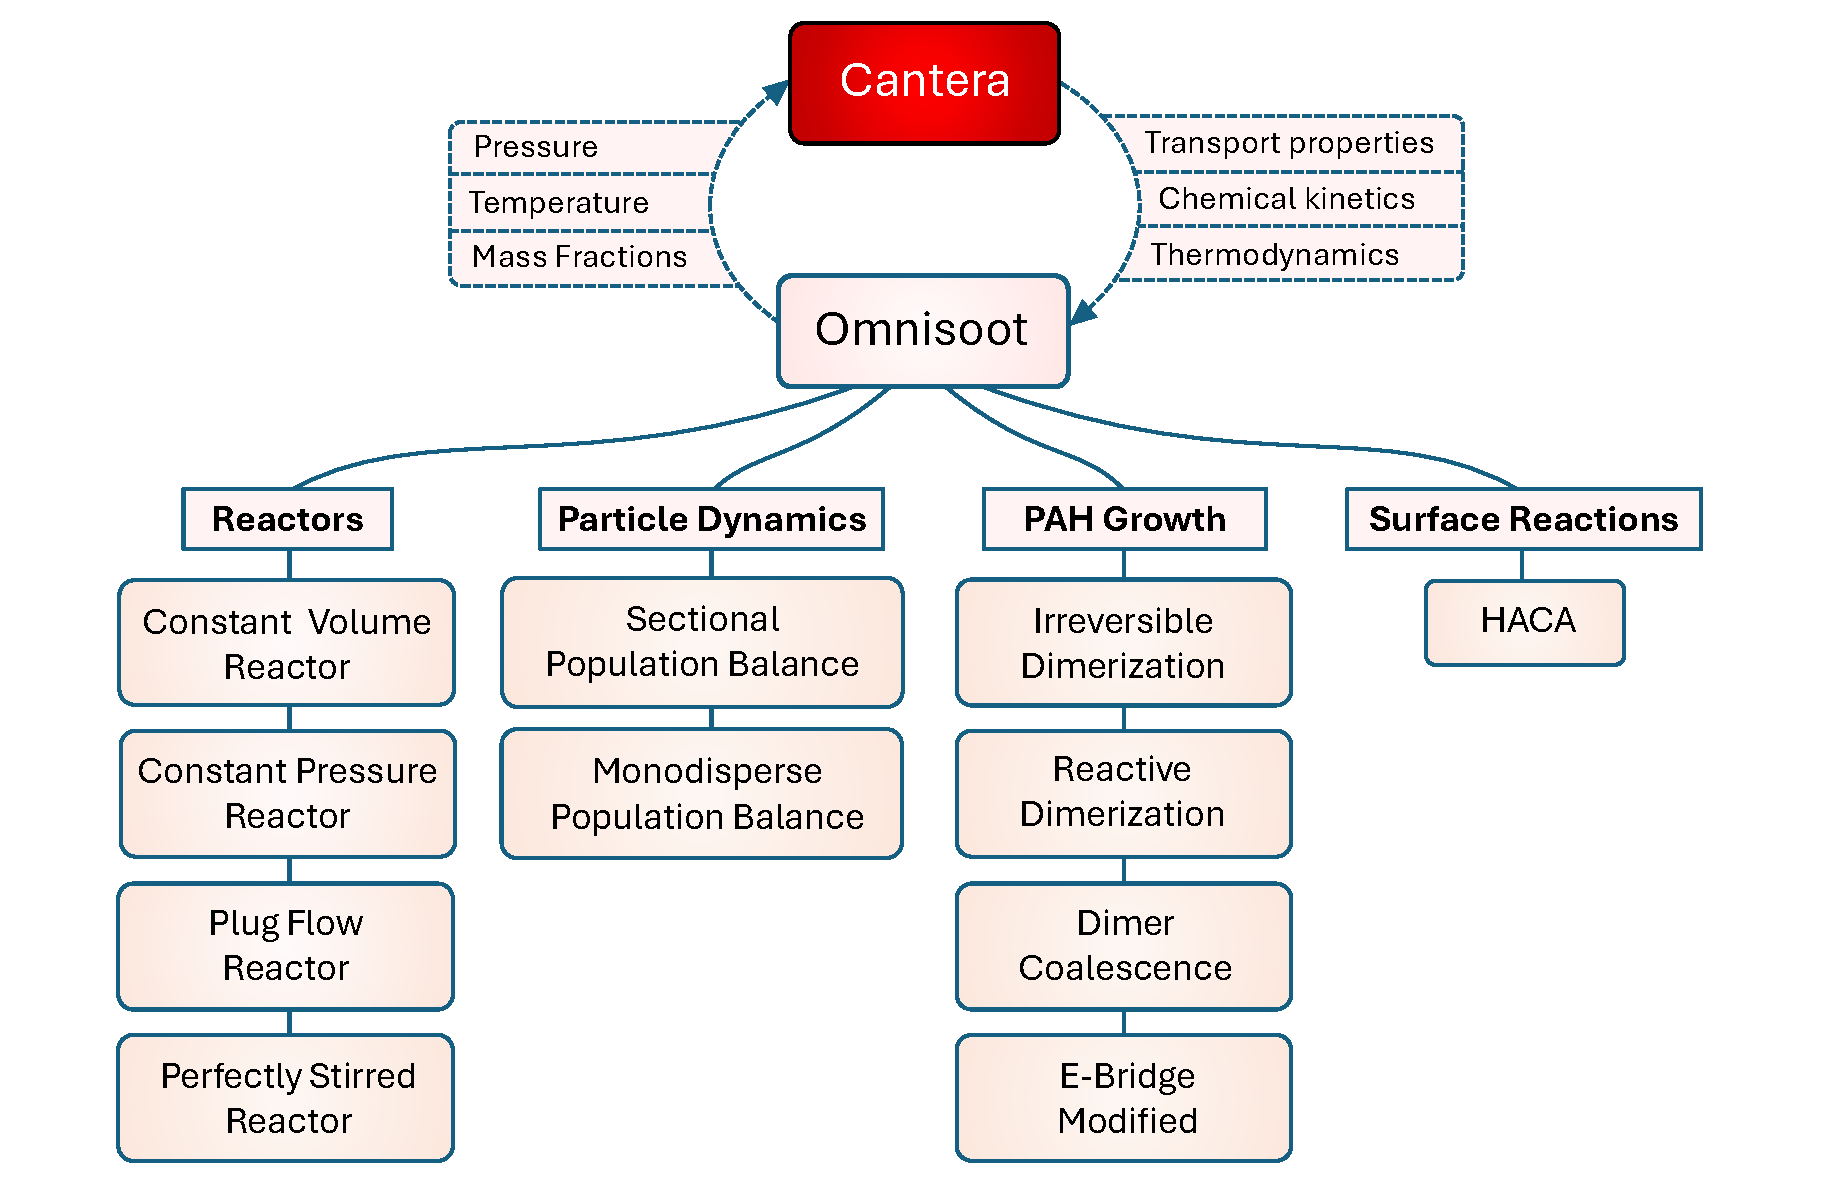
\includegraphics[height=90mm, ]{Figures/Theory/structure.pdf}
	\caption{The structure of Omnisoot that illustrates the coupling with Cantera and sub-models including reactors, particle dynamic models, PAH growth models and surface reactions models}
	\label{fig:structure}
\end{figure}


\section{Assumptions and conventions}
Here, the main conventions and assumptions used in the derivation of the mathematical models are listed below.

\begin{enumerate}
	%\item The ideal gas law is used to calculated physical, transport, and chemical properties of gas mixtures.
	
	\item $f_v$ and $\varphi$ denote the volume of soot particles normalized by the gas volume and reactor volume, respectively. Their relationship can be expressed as:
	
	\begin{equation}
		\begin{split}
			f_v = \frac{V_{soot}}{V_{gas}}, \\
			\varphi = \frac{V_{soot}}{V_{gas} + V_{soot}}, \\
			\varphi = \frac{f_v}{1 + f_v}
			\label{eqn:fvdef}.
		\end{split}
	\end{equation}
	
	\item ${\dot{s}_k}$ denotes the rate production/consumption of $k_{th}$ gaseous species (i.e., gas scrubbing) due to soot inception, surface growth and oxidation. It is positive when the species is released to the gas mixture.
	
	\item Each soot agglomerate consists of monodisperse spherical primary particles, which are in point contact. So, the model does not consider formation of necking (or sintering) in soot agglomerates by surface growth.
	
	%\item The primary particles of each agglomerate are similar enough that can be described by mean size and composition.
	
	\item The word \textit{``particle"} refers to soot both in spherical and agglomerate shape. 
	
	\item The density of soot is assumed constant at the value of 1800 $\mathrm{kg/m^3}$. Soot density changes with its maturity level, which is often linked to the elemental C/H ratio of soot particles~\citep{michelsen2021effects}. Here, the considered value represents an average between density of mature soot with high C/H ratios ($\mathrm{\rho=2000\;kg/m^3}$) and that of nascent soot with low C/H ratios ($\mathrm{\rho=1600\;kg/m^3}$)~\citep{jensen2007measurement, michelsen2021effects}.
	
	\item The incipient soot particles are 2~nm in diameter, so the model does not allow particles with a primary particle diameter smaller than 2~nm. The number of carbon atoms in the incipient soot particle, $n_{c,min}$, is calculated from the mass of a sphere with a diameter of $d_{p,min}=2$~nm assuming pure carbon content, which results in:
	\begin{equation}
		\begin{split}
			n_{c,min}& =\frac{\pi}{6}\rho_{soot}d^3_{p,min}\frac{1}{W_{carbon}}\approx378.
			\label{eqn:nc_min}
		\end{split}
	\end{equation}
	
	
	\item The specific heat, internal energy and enthalpy of soot are approximated by those of pure graphite, and are employed to close the energy balance in the system~\cite{mcbride1993coefficients}.
	
	\item Soot particles and gas are in thermal equilibrium during soot formation processes, and there is no temperature gradient within each agglomerate.
	
	
	\item $\psi$ denotes a \textit{soot variable} that represents a mean property of soot particles in each section tracked in Omnisoot by solving transport equations for the total concentration of agglomerates, $N_{agg}$ and primary particles, $N_{pri}$, and the total carbon, $C_{tot}$ and hydrogen content, $H_{tot}$ of soot. $S_{\psi}$ is the source term of the soot variable, $\psi$, which appears in soot equations.  
	
	\item \textit{PAH growth} is a sub-model of Omnisoot with a set of pathways that determine the rate of inception and adsorption from PAHs (designated as soot precursors) in the gas mixture.
	
	\item \textit{Surface reactions} is a sub-model of Omnisoot that describes the addition of acetylene to soot surface, and removal of carbon via oxidation by OH and $\mathrm{O_2}$ following the HACA scheme. The model does not consider soot oxidation with $\mathrm{CO_2}$, $\mathrm{H_2O}$ and $\mathrm{NO_x}$.
	
	\item The single superscript \textit{i} denotes the section number of a soot variable or a derived property. For example, $d^i_p$ represents the primary particle diameter of section \textit{i}. The double superscript \textit{ij} indicates a property related to two sections; for example, $\beta^{ij}$ denotes the collision frequency between sections \textit{i} and \textit{j}. In the case of the monodisperse model, the section number can be omitted because it is equivalent to the sectional model with only one section.
	
	
	\item The computation of morphological parameters is done similarly in both particle dynamics models, but they are explained separately in Section~\ref{sec:sootmorphology}.
	
	\item \textit{precursors} refer to the PAHs larger than naphthalene used for inception and PAH adsorption. The list of precursors with their chemical formula and molecular mass is provided in Table~\ref{tab:precursors_list}. It should be noted that the precursors can be dynamically changed by Omnisoot's user interface.
	
	\renewcommand{\arraystretch}{1.5}
	\begin{table}
		\caption{The names, symbols, chemical formula and molecular weight of the soot precursors used by Omnisoot.}
		\label{tab:precursors_list}
		\centering
		\begin{tabular}{l l l l}
			\hline
			Species name & Symbol & Chemical formula & W~[kg/mol] \\
			\hline
			Naphthalene       & A2   &  $\mathrm{C_{10}H_{8}}$   & 0.128 \\
			Phenanthrene      & A3   &  $\mathrm{C_{14}H_{10}}$  & 0.178 \\
			Pyrene            & A4   &  $\mathrm{C_{16}H_{10}}$  & 0.202 \\
			Acenaphthylene    & A2R5 &  $\mathrm{C_{12}H_{8}}$   & 0.152 \\
			Acephenanthrylene & A3R5 &  $\mathrm{C_{16}H_{10}}$  & 0.202 \\
			Cyclopentapyrene  & A4R5 &  $\mathrm{C_{18}H_{10}}$  & 0.226 \\
			\hline
		\end{tabular}
	\end{table}
	
\end{enumerate}

